\subsection{Benchmarks}
\label{subsec:exp3}
In this section, we present the results obtained through the experiments on some efficiency aspects of generated code to answer the following question.

%\noindent
%\tb{\ti{Research question 2:}} \ti{Runtime performance and memory usage is undoubtedly critical in real-time and embedded systems. 
%Particularly, in event-driven systems, the performance is measured by event processing speed. 
%Is the performance of code generated by our tool comparable existing approaches and use less memory?}


\begin{mdframed}[backgroundcolor=blue!5]
\small
\tb{\ti{Research question 2:}} \ti{Runtime performance and memory usage are undoubtedly critical in real-time and embedded systems. 
Particularly, in event-driven systems, the performance is measured by event processing speed. 
Are the performance and memory usage of code generated by our tool comparable to existing approaches?}
\end{mdframed}
%Specifically, our research question related to memory consumption and runtime performance of generated code is stated as the following. 
%\noindent
%\tb{RQ3:} \ti{}
%\noindent
%\tb{Experimental dataset:} 
Two state machine examples are obtained by the preferred benchmark used by the Boost C++ libraries \cite{boost} in \cite{benchmark}. One simple example only consists of atomic states and the other both atomic and composite states. 

We compared our tool with tools such as Sinelabore (which generates efficient code for Magic Draw \cite{Magicdraw}, Enterprise Architect \cite{EA}), Quantum Modeling (QM) \cite{qm} (which generates code for event-driven active object frameworks \cite{Lavender1996})%, which generate code from state machines
, Boost Statechart \cite{Statechart}, Meta State Machine (MSM) \cite{MSM}, C++ 14 MSM-Lite \cite{benchmark}, and functional programming like-EUML\cite{EUML}. 
%The tools are Sinelabore, which efficiently generates code from UML State Machines created by various modeling tools such as Magic Draw \cite{Magicdraw}, Enterprise Architect \cite{EA}, and QM \cite{QM}. 
%C++ libraries are Boost Statechart \cite{Statechart}, Meta State Machine (MSM) \cite{MSM}, MSM-Lite \cite{MSMLite}, and EUML \cite{euml}.

We used a Ubuntu virtual machine 64 bit hosted by a Windows 7 machine. 
For each tool, we created two applications corresponding to the two examples, generated C++ code and compiled it in two modes: normal (N), by default GCC compiler; and optimal (O) with GCC optimization options -O2 -s. 
11 millions of events are generated and processed by the simple example and more than 4 millions for the composite example. 
%More than 4 millions of events are processed by the composite example. 
Processing time is measured for each case. 

\subsubsection{Performance} 
Fig. \ref{fig:boxplot} shows the event processing performance of the approaches for the two benchmarks.
%Table \ref{table-speed} shows the median of event processing time. 
In the normal compilation mode ( postfix N), Boost Statechart, MSM, MSMLite, EUML are quite slow and not displayed in the box-plot. 
%Only Sinelabore and QM are performantly comparable with our approach. 
  
%Boxplots in Fig. \ref{fig:boxplotsimple} and \ref{fig:boxplotcomposite} compare the performance of these approaches to that of our approach for the two examples, respectively. 
%In both of the simple and composite examples, 

%Our approach processes faster around 40 milliseconds than the fastest approach within the scope of the experiment.
%Even without GCC optimizations, code generated by our approach significantly runs faster than that of EUML and QM with the optimizations. 
%When compiled with the optimizations, our approach improves the event processing speed. 
In both of the simple and composite benchmarks, in optimization mode (postfix O) MSMLite and our tool run faster than the others in the scope of the experiment.
The figure also shows that the optimization of GCC is significant.
In normal mode only the performance of Sinelabore, QM, and our tool is acceptable. 
The event processing speed of MSM, MSM\_Lite and EUML is too slow without GCC optimizations. 
%Even, in case of composite, our approach does not produce any slowness compared to the simple example. 


% Please add the following required packages to your document preamble:
% \usepackage{multirow}
\begin{comment}
\begin{table*}[]
	\centering
	\caption{Event processing speed in ms}
\label{my-label}
\begin{tabular}{|l|l|l|l|l|l|l|l|l|l|l|l|l|l|l|l|l|}
	\hline
	\multicolumn{1}{|c|}{\multirow{2}{*}{Test}} & \multicolumn{2}{c|}{SC} & \multicolumn{2}{c|}{MSM} & \multicolumn{2}{c|}{MSM-Lite} & \multicolumn{2}{c|}{EUML} & \multicolumn{2}{c|}{Sinelabore} & \multicolumn{2}{c|}{QM} & \multicolumn{2}{l|}{Umple} & \multicolumn{2}{c|}{Our approach} \\ \cline{2-17} 
	\multicolumn{1}{|c|}{}                      & N           & O         & N            & O         & N              & O            & N            & O          & N               & O             & N          & O          & N            & O           & N                & O              \\ \hline
	Simple                                      & 13705,75    & 1658,1    & 5249,57      & 70,63     & 833,67         & 79,37        & 10867,93     & 109,97     & 141,03          & 79,93         & 285,9      & 229,27     & X            & X           & 106,87           & 25,37          \\ \hline
	Composite                                   & 5353,03     & 820,63    & 3546,1       & 46,73     & 516,87         & 65,17        & 4225,57      & 92,3       & 100,03          & 86,03         & 146,23     & 97,57      & X            & X           & 36,47            & 1,40           \\ \hline
\end{tabular}
\end{table*}
\end{comment}

\begin{comment}
\begin{table*}[]
	\centering
	\caption{Event processing speed in ms}
	\label{table-speed}
	\begin{tabular}{|l|l|l|l|l|l|l|l|l|l|l|l|l|l|l|l|l|}
		\hline
		\multicolumn{1}{|c|}{\multirow{2}{*}{Test}} & \multicolumn{2}{c|}{SC} & \multicolumn{2}{c|}{MSM} & \multicolumn{2}{c|}{MSM-Lite} & \multicolumn{2}{c|}{EUML} & \multicolumn{2}{c|}{Sinelabore} & \multicolumn{2}{c|}{QM} & \multicolumn{2}{l|}{Umple} & \multicolumn{2}{c|}{Our approach} \\ \cline{2-17} 
		\multicolumn{1}{|c|}{}                      & N           & O         & N            & O         & N              & O            & N            & O          & N               & O             & N          & O          & N            & O           & N                & O              \\ \hline
		Simple                                      & 13706    & 1658    & 5250      & 71     & 834         & 79        & 10868     & 110     & 141          & 80         & 286      & 229     & X            & X           & 107           & 25,4          \\ \hline
		Composite                                   & 5353     & 821    & 3546       & 47     & 517         & 65        & 4225,6      & 92       & 100          & 86         & 146     & 98      & X            & X           & 36,5            & 1,40           \\ \hline
	\end{tabular}
\end{table*}
\end{comment}


\begin{comment}
\begin{table*}[]
	\centering
	\caption{Event processing speed in ms}
	\label{table-speed}
	\begin{tabular}{|l|l|l|l|l|l|l|l|l|l|l|l|l|l|l|}
		\hline
		\multicolumn{1}{|c|}{\multirow{2}{*}{Test}} & \multicolumn{2}{c|}{SC} & \multicolumn{2}{c|}{MSM} & \multicolumn{2}{c|}{MSM-Lite} & \multicolumn{2}{c|}{EUML} & \multicolumn{2}{c|}{Sinelabore} & \multicolumn{2}{c|}{QM} & \multicolumn{2}{c|}{PSM} \\ \cline{2-15} 
		\multicolumn{1}{|c|}{}                      & N           & O         & N            & O         & N              & O            & N             & O         & N               & O             & N          & O          & N           & O          \\ \hline
		Simple                                      & 13706       & 1658      & 5250         & 71        & 834            & 79           & 10868         & 110       & 141             & 80            & 286        & 229        & 107         & 25,4       \\ \hline
		Composite                                   & 5353        & 821       & 3546         & 47        & 517            & 65           & 4225,6        & 92        & 100             & 86            & 146        & 98         & 36,5        & 1,40       \\ \hline
	\end{tabular}
\end{table*}
\end{coment}


\begin{comment}
\begin{figure}
	\centering
	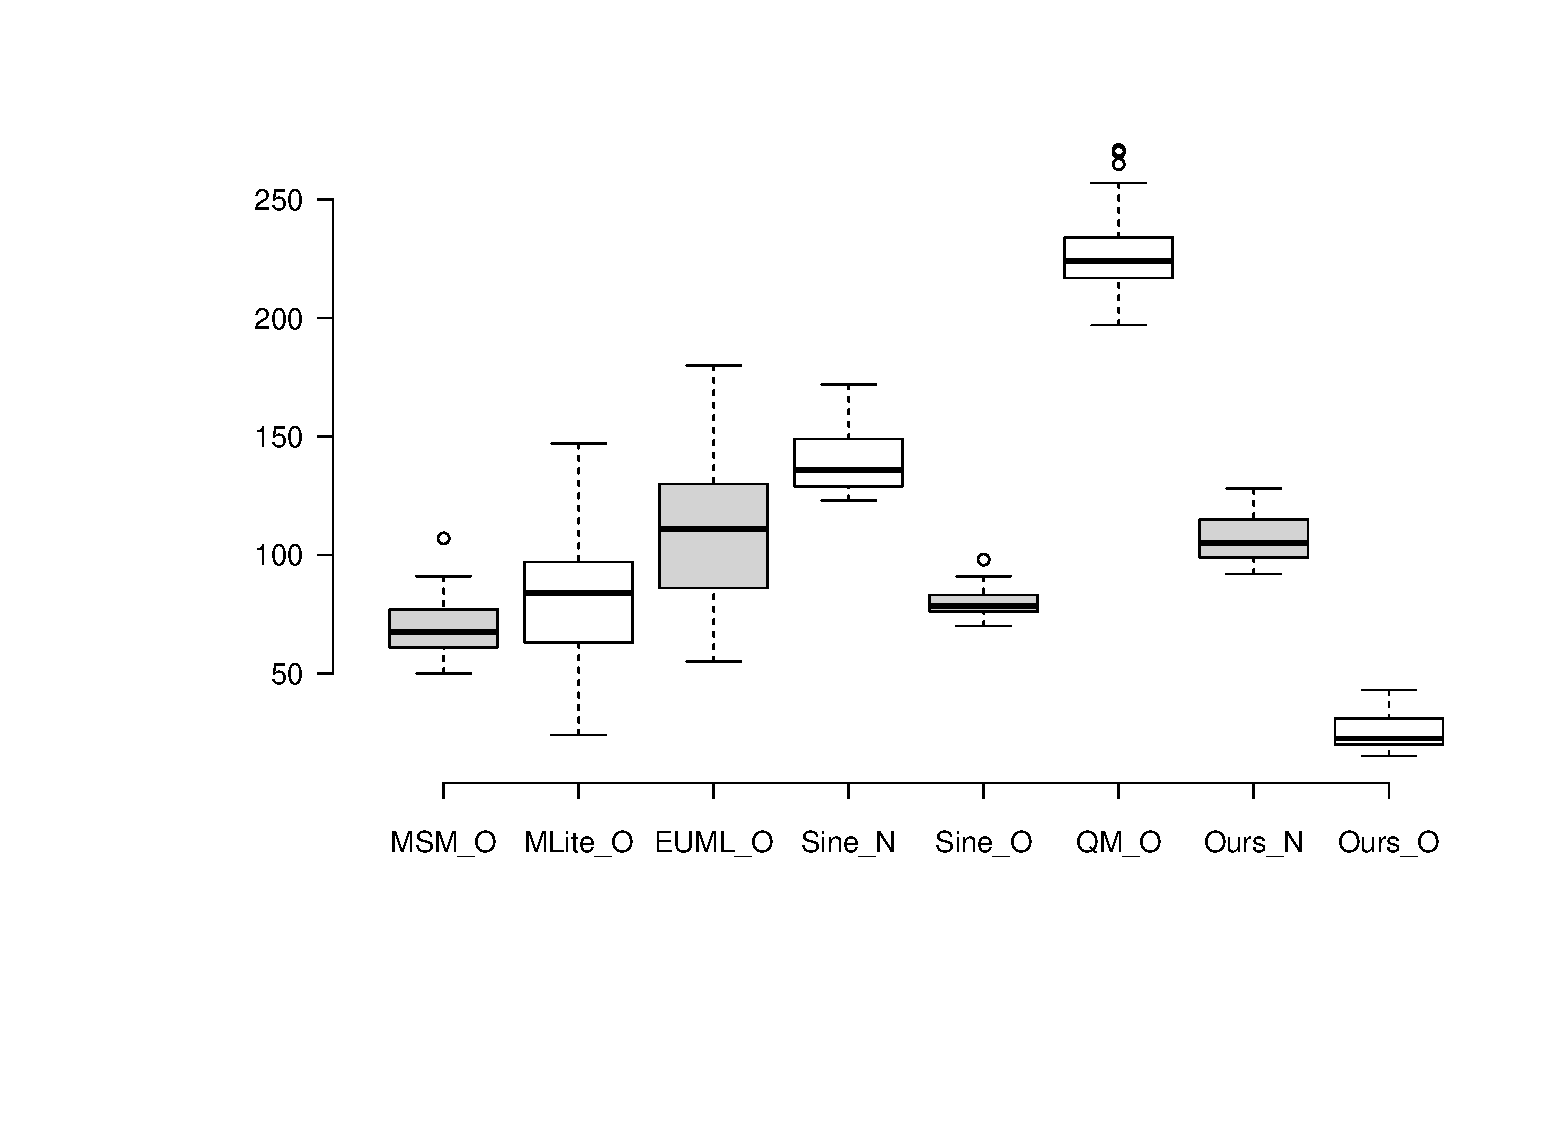
\includegraphics[clip, trim=4.2cm 4.6cm 1.7cm 2.3cm, width=\columnwidth]{figures/boxplotsimple.pdf}
	\caption{Event processing speed for the \ti{Simple} benchmark} 
	\label{fig:boxplotsimple}
\end{figure}

\begin{figure}
	\centering
	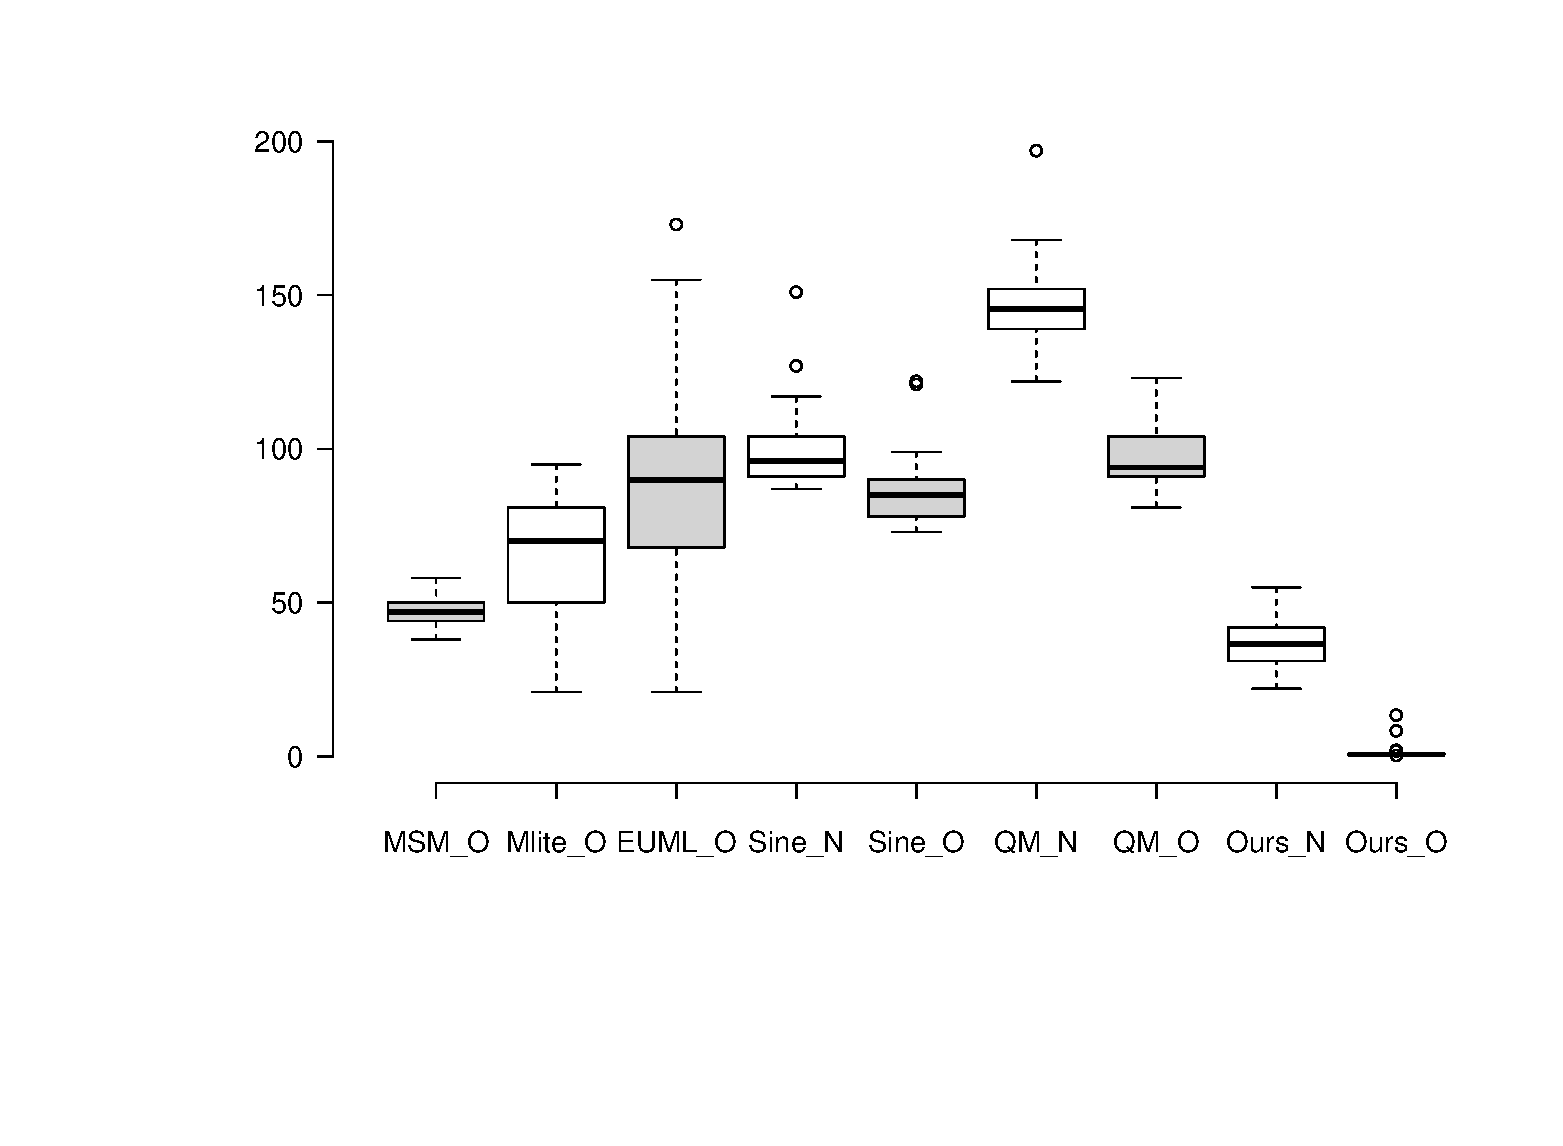
\includegraphics[clip, trim=4.2cm 4.6cm 1.7cm 1.8cm, width=\columnwidth]{figures/boxplotcomposite.pdf}
	\caption{Event processing speed for the \ti{Composite} benchmark} 
	\label{fig:boxplotcomposite}
\end{figure}
\end{comment}

\begin{figure}
	\centering
	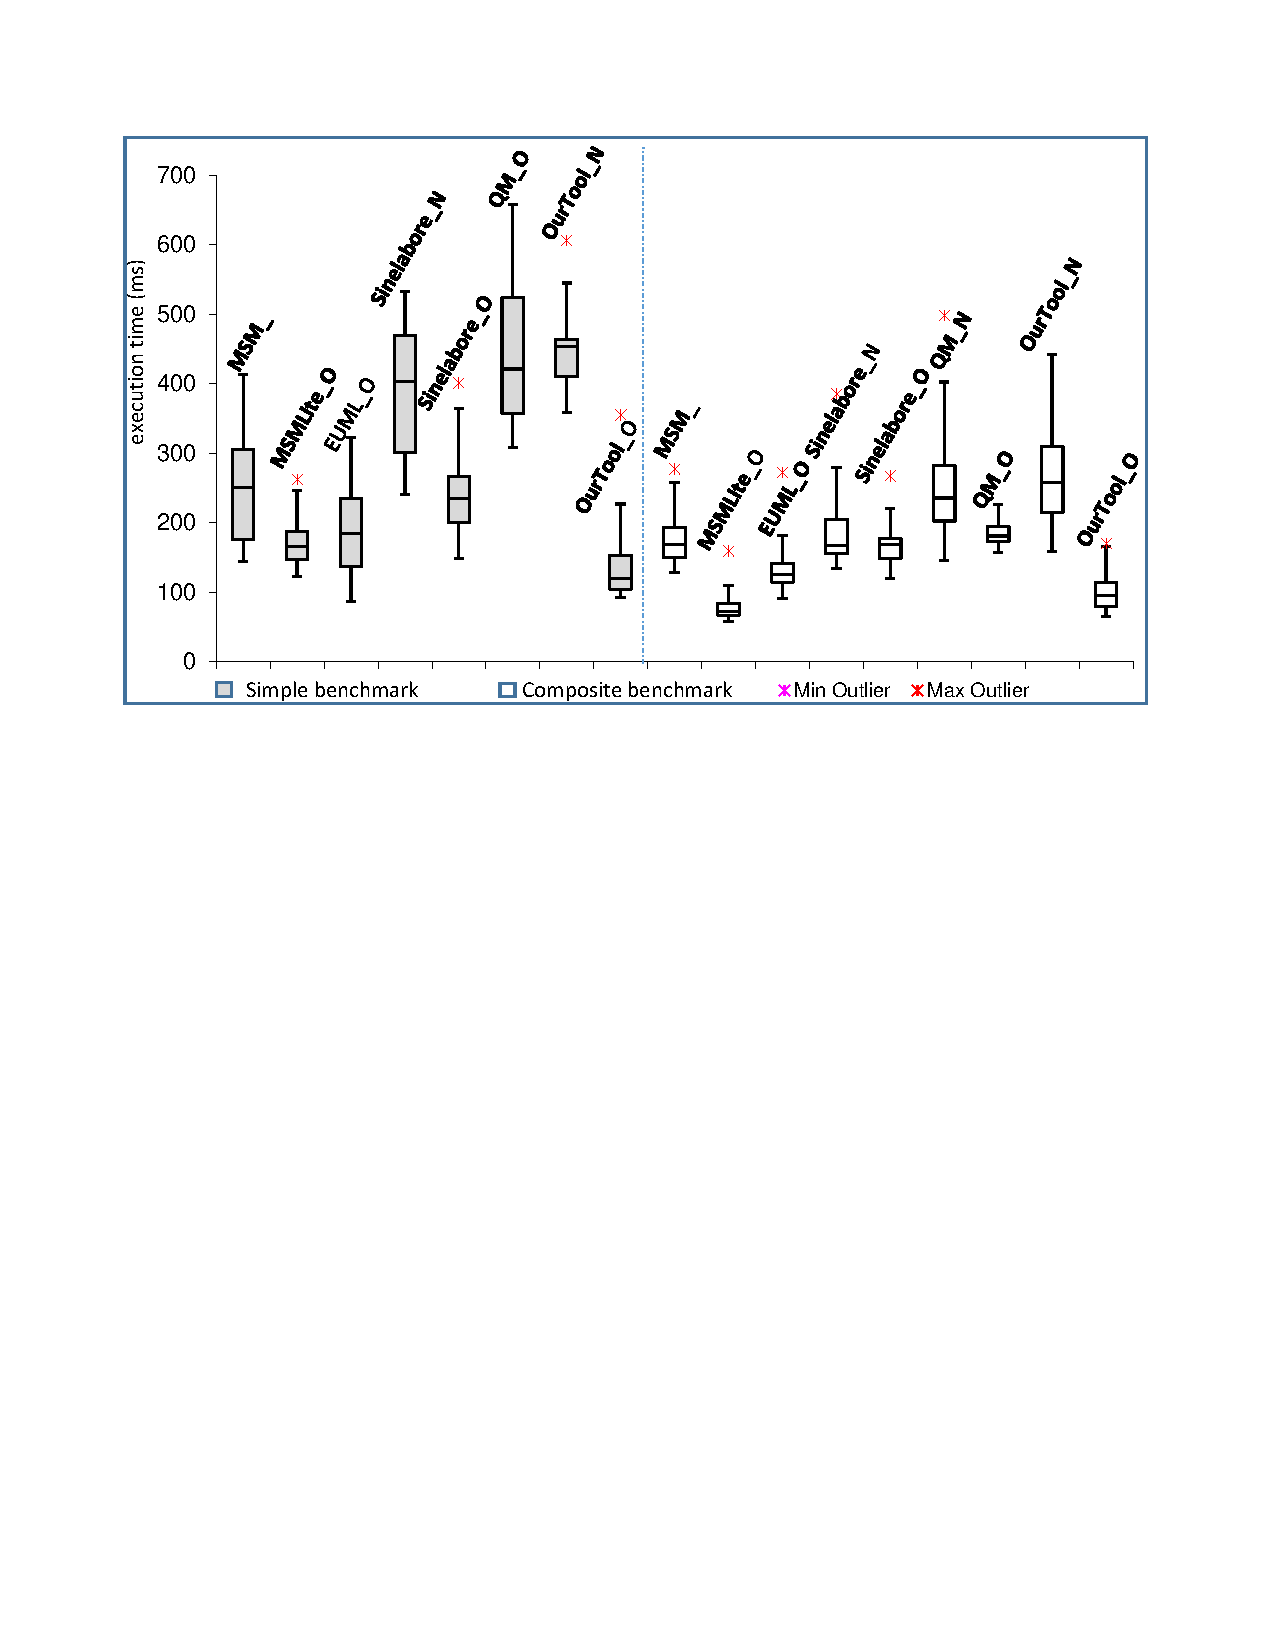
\includegraphics[clip, trim=2.1cm 16.0cm 1.7cm 2.3cm, width=\columnwidth]{experiments/box-plot-mine.pdf}
	\caption{Event processing speed for the benchmarks} 
	\label{fig:boxplot}
\end{figure}

\subsubsection{Memory usage} 
Table \ref{table-size} shows the executable size for the examples compiled in two modes.
Without optimization, Sinelabore generates the smallest executable size while our approach takes the second place.
In GCC optimization mode, MSMLite, Sinelabore and our approach require less static memory than the others. 

Let's look closer at the event processing performance in optimization mode in terms of time medians.
Fig. \ref{fig:comparepercentage} shows the figures of the two benchmarks, relative to the performance of Sinelabore (normalized to 100\%).
For the simple (blue) benchmark, our approach (51.3\%) is the fastest. 
For the composite (red) benchmark, with the support of C++14, the performance in MSMLite (42.7\%) is the fastest and ours is the second.   

For runtime memory consumption, we use the Valgrind Massif profiler \cite{Massif,nethercote2007valgrind} to measure memory usage. 
Table \ref{table:usage} shows the memory consumption measurements including stack and heap usage for the composite example. 
Compared to others, code generated by our approach requires a slight overhead with regard to runtime memory usage (0.35KB).
This is predictable since the major part of the overhead is used for C++ multi-threading using POSIX Threads and resource control using POSIX Mutex and Condition. 
However, the overhead is small and acceptable (0.35KB). 


\begin{comment}
\begin{table*}[]
	\centering
	\caption{Executable size in Kb}
	\label{table-size}
	\begin{tabular}{|l|l|l|l|l|l|l|l|l|l|l|l|l|l|l|l|l|}
		\hline
		\multirow{2}{*}{Test} & \multicolumn{2}{c|}{SC} & \multicolumn{2}{c|}{MSM} & \multicolumn{2}{c|}{MSM-Lite} & \multicolumn{2}{c|}{EUML} & \multicolumn{2}{c|}{Sinelabore} & \multicolumn{2}{c|}{QM} & \multicolumn{2}{l|}{Umple} & \multicolumn{2}{c|}{Our approach} \\ \cline{2-17} 
		& N           & O         & N           & O          & N              & O            & N            & O          & N              & O              & N          & O          & N            & O           & N               & O               \\ \hline
		Simple                & 320      & 63,9     & 414,6      & 22,9      & 107,3         & 10,6        & 2339      & 67,9      & 16,5          & 10,6          & 22,6      & 10,5      &       X       &       X      & 21,5           & 10,6           \\ \hline
		Composite             & 435,8      & 84,4     & 837,4      & 31,1      & 159,2         & 10,9        & 4304,8      & 92,5      & 16,6          & 10,6          & 23,4      & 21,5      & X           & X          & 21,6           & 10,6           \\ \hline
	\end{tabular}
\end{table*}
\end{comment}


%ToDo: test speed with dispatch function
% Please add the following required packages to your document preamble:
% \usepackage{multirow}
\begin{table*}[]
	\scriptsize
	\centering
	\caption{Executable size in KB}
	\label{table-size}
	\begin{tabular}{|l|l|l|l|l|l|l|l|l|l|l|l|l|}
		\hline
		\multirow{2}{*}{Test} & \multicolumn{2}{c|}{MSM} & \multicolumn{2}{c|}{MSM-Lite} & \multicolumn{2}{c|}{EUML} & \multicolumn{2}{c|}{Sinelabore} & \multicolumn{2}{c|}{QM} & \multicolumn{2}{c|}{Our tool} \\ \cline{2-13} 
		& N           & O          & N              & O            & N            & O          & N              & O              & N          & O          & N            & O           \\ \hline
		Simple                & 414,6       & 22,9       & 107,3          & 10,6         & 2339         & 67,9       & 16,5           & 10,6           & 22,6       & 16,6       & 21,5         & 10,6        \\ \hline
		Composite             & 837,4       & 31,1       & 159,2          & 10,9         & 4304,8       & 92,5       & 16,6           & 10,6           & 23,4       & 21,5       & 21,6         & 10,6        \\ \hline
	\end{tabular}
\end{table*}

%\subsubsection{Runtime memory consumption}
\begin{comment}
\begin{table}[]
	\centering
	\caption{Runtime memory consumption in KB. Columns (1) to (7) are SC, MSM, MSM-Lite, EUML, Sinelabore, QM, and our approach, respectively.}
	\label{table:usage}
	\begin{tabular}{|l|l|l|l|l|l|l|l|l|}
		\hline
		Test      & (1)    & (2)  & (3) & (4) & \begin{tabular}[c]{@{}l@{}}(5)\end{tabular} & (6)    & \begin{tabular}[c]{@{}l@{}}(7)\end{tabular} \\ \hline
		Composite & 76.03 & 75.5 & 75.8  & 75.5 & 75.8                                                  & 75.7      & 76.38                                                   \\ \hline
	\end{tabular}
\end{table}
\end{comment}

\begin{table}[]
	\scriptsize
	\centering
	\caption{Runtime memory consumption in KB. Columns from left to right are SC, MSM, MSM-Lite, EUML, Sinelabore, QM, and Our tool, respectively.}
	\label{table:usage}
	\begin{tabular}{|l|l|l|l|l|l|l|}
		\hline
		76.03 & 75.5 & 75.8 & 75.5 & 75.8 & 75.7 & 76.38 \\ \hline
	\end{tabular}
\end{table}


\begin{figure}
	\centering
	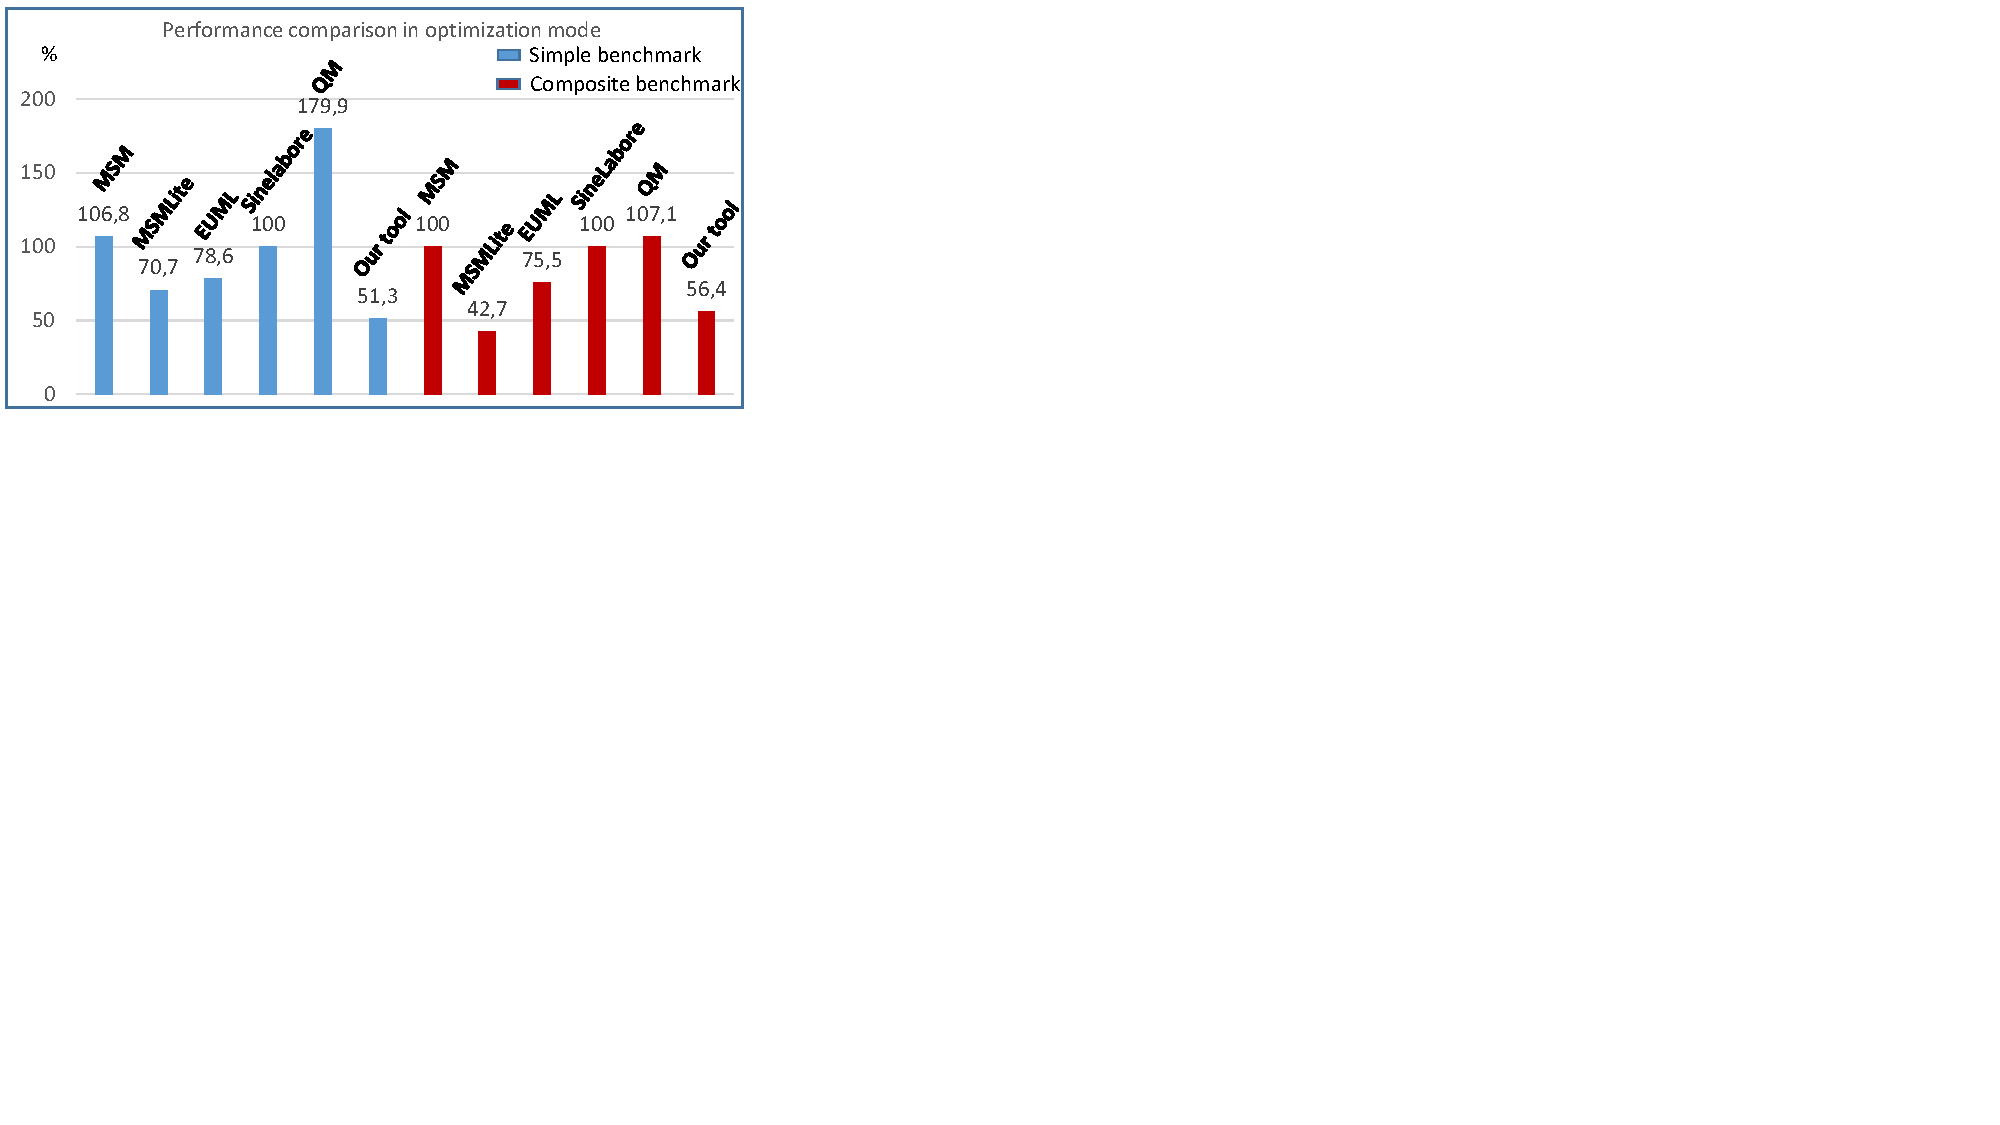
\includegraphics[clip, trim=0cm 12.1cm 21.0cm 0cm, width=\columnwidth]{experiments/comparepercentage.pdf}
	\caption{Event processing performance in optimization mode} 
	\label{fig:comparepercentage}
\end{figure}


%\lipsum[1-6]